\subsection{Bicycle model of a car}

\begin{figure}
\centering
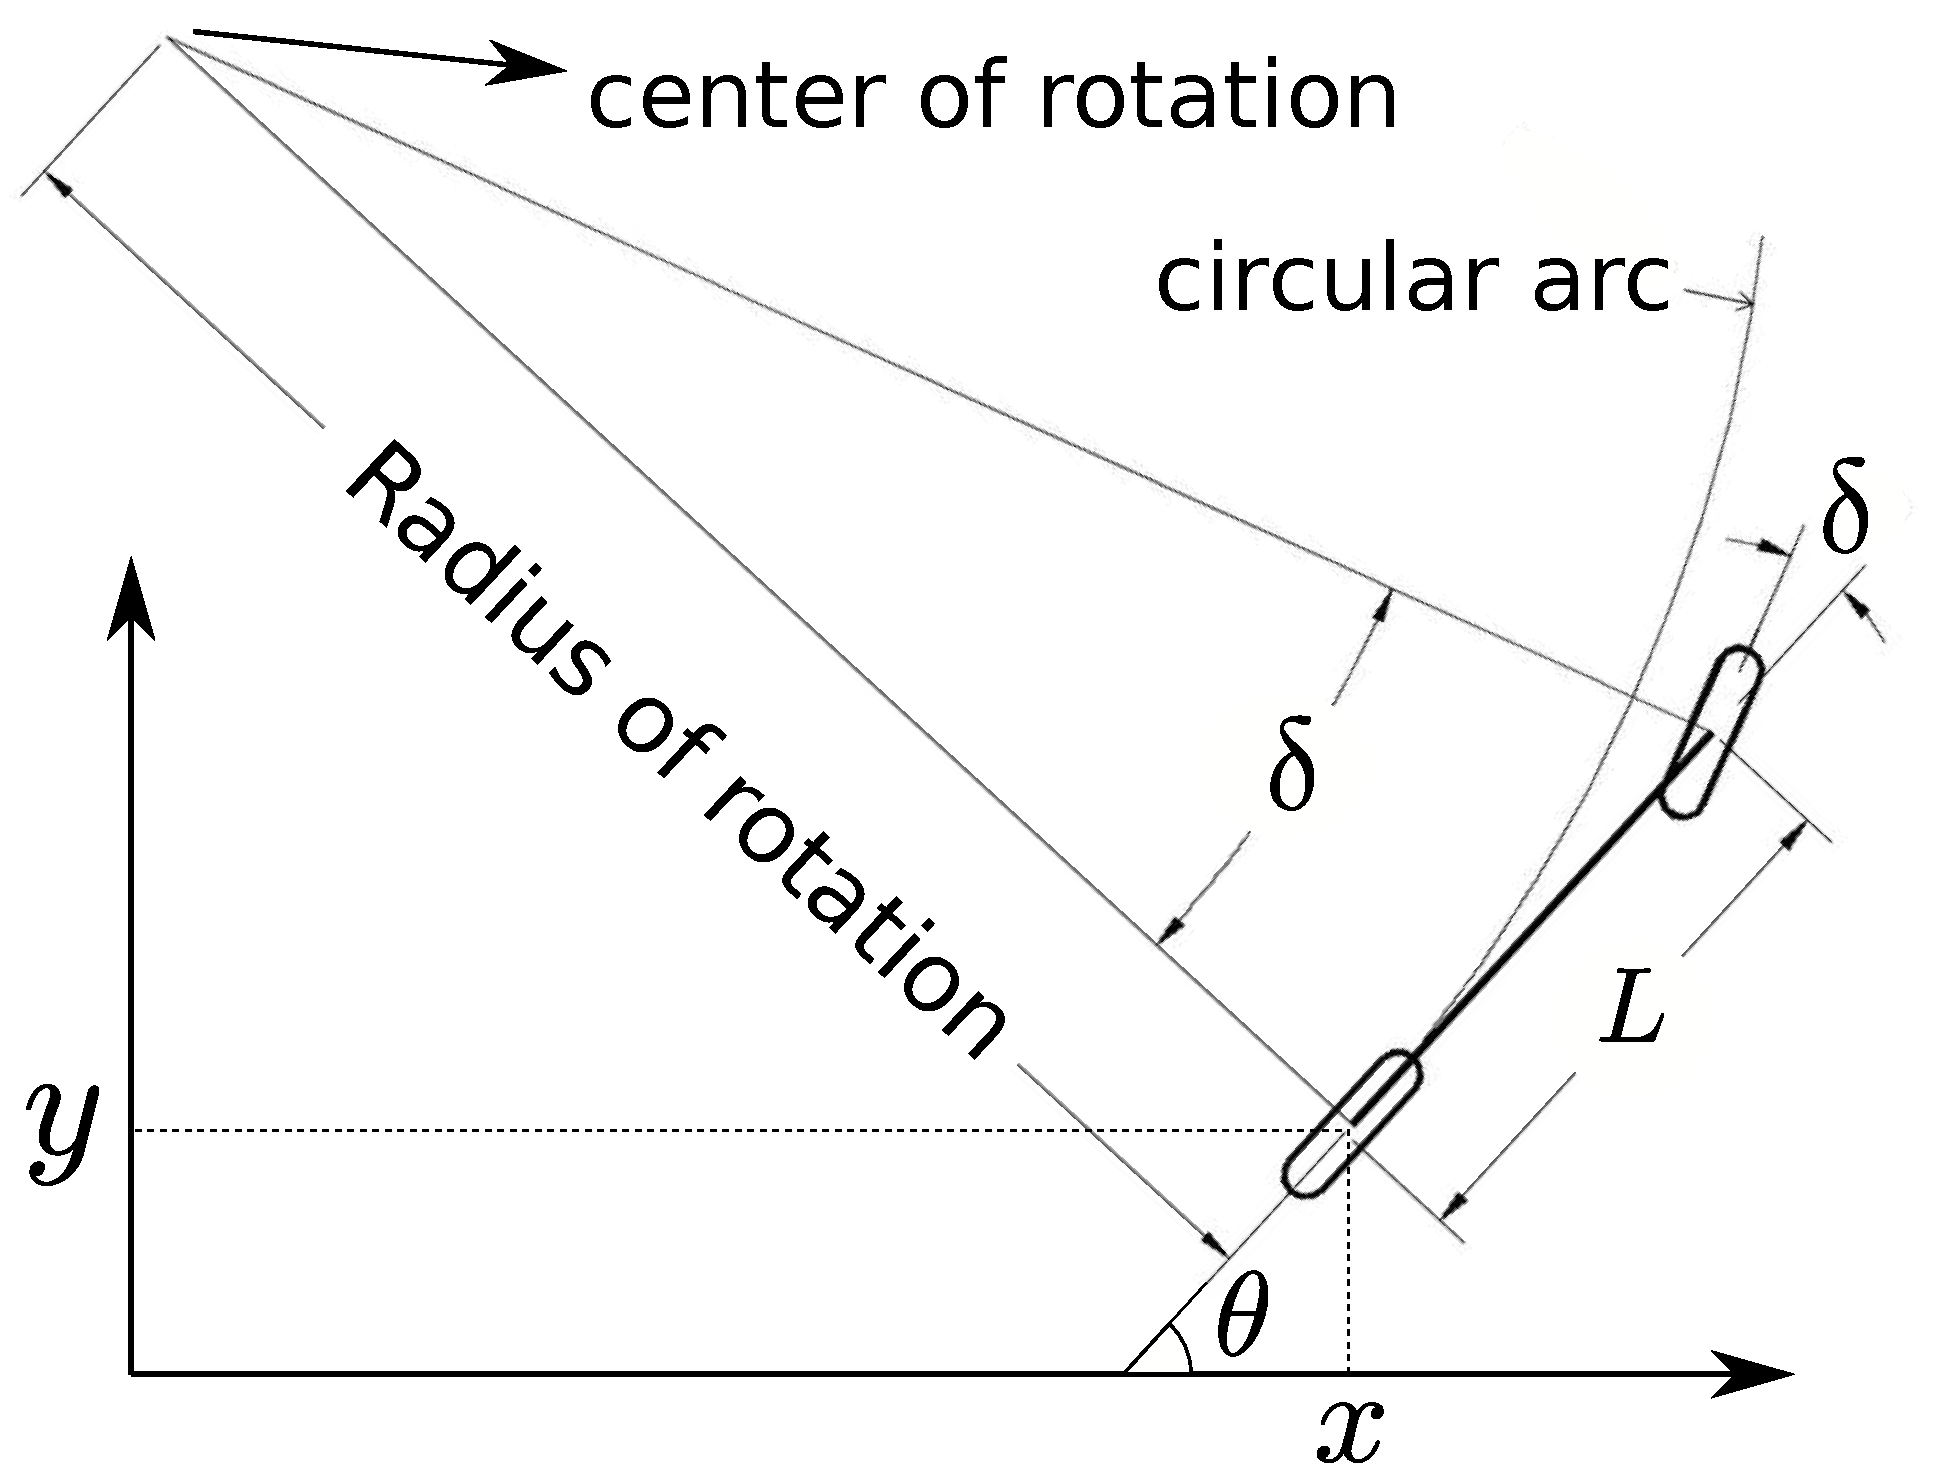
\includegraphics[width=45mm]{Figures/BicycleModel-coords.pdf}%
\caption{Bicycle model \cite{Snider.2009}}
\label{fig:bicycle}%
\end{figure}

Our formal analysis is based on the
bicycle model of a car, where we imagine that there is one rear wheel at the center of the rear axle and one front wheel at the center of the front axle.
We assume no wheel slippage, and only the front wheel can steer.
This model defines a dynamical system.
The \emph{state} of the system at time $t$
is described by the triple $(x(t), y(t), \theta(t))$
where $(x, y)$ are the coordinates of the rear wheel
in some inertial frame, say the racing track, and
$\theta$ is the angle of the heading direction of the bicycle measured from the $x$-axis counter-clockwise.
If $v$ is the speed (magnitude of velocity) of the rear wheel,
$L$ is the \emph{wheelbase} (distance between the rear and front wheels),
and $\delta$ is the steering angle,
then
\[
\left\{
\begin{array}{l}
     \dot{x} = v \cdot cos(\theta) \\
     \dot{y} = v \cdot sin(\theta) \\
     \dot{\theta} = \frac{\displaystyle v}{L} tan(\delta)
\end{array}
\right.
\]

Illustration of the bicycle model of the vehicle is provided in Figure~\ref{fig:bicycle}.
